% % % % % % % % % % % % % % % % % % % % % % % % % % % % % % % % % % % % % % % % % % % %
%                                                                                     %
% Short Sectioned Assignment LaTeX Template Version 1.0 (5/5/12)                      %
% This template has been downloaded from: http://www.LaTeXTemplates.com               %
%                                                                                     %
% Original author:  Frits Wenneker (http://www.howtotex.com)                          %
%                                                                                     %
% Modified by: Fco Javier Sueza Rodríguez (fcosueza@disroot.org)                      %
%                                                                                     %
% Changes:                                                                            %
%	    - Custom Chapters, Sections and Subsections (titlesec package)                %
%           - Document type scrbook (oneside)                                         %
%           - Use babel-lang-spanish package and marvosym                             %
%           - Use hyperref, enumitem, tcolorbox and glossaries packages               %
%           - Use Time New Roman (mathptmx), Helvetic and Courier fonts               %
%                                                                                     %
% License: CC BY-NC-SA 3.0 (http://creativecommons.org/licenses/by-nc-sa/3.0/)        %
%                                                                                     %
% % % % % % % % % % % % % % % % % % % % % % % % % % % % % % % % % % % % % % % % % % % %

%-----------------------------------------------%
%	              Packages                  %
%-----------------------------------------------%

\documentclass[paper=a4, fontsize=11pt, oneside]{scrbook}

% ---- Text Input/Output ----- %

\usepackage[T1]{fontenc}
\usepackage[utf8]{inputenc}
\usepackage{mathptmx}
\usepackage[scaled=.92]{helvet}
\usepackage{courier}
\usepackage[indent=12pt]{parskip}

\usepackage{geometry}
\geometry{verbose,tmargin=3cm,bmargin=3cm,lmargin=2.6cm,rmargin=2.6cm}

% ---- Language ----- %

\usepackage[spanish]{babel}
\usepackage{marvosym}

% ---- Another packages ---- %

\usepackage{amsmath,amsfonts,amsthm}
\usepackage{graphics,graphicx}
\usepackage{titlesec}
\usepackage{fancyhdr}
\usepackage{tcolorbox}
\usepackage{hyperref}
\usepackage{enumitem}
\usepackage[automake]{glossaries}

%--------------------------------------------------------------------%
%                      Customizing Document                          %
%--------------------------------------------------------------------%


% ----------- Custom Chapters, Sections and Subsections -------------- %

\titleformat{\chapter}[display]
			{\bfseries\Huge}
			{Tema \ \thechapter} {0.5ex}
			{\vspace{1ex}\centering}

\titleformat{\section}[hang]
			{\bfseries\Large}
			{\thesection}{0.5em}{}

\titleformat{\subsection}[hang]
			{\bfseries\large}
			{\thesubsection}{0.5em}{}

\titleformat{\subsubsection}[hang]
			{\bfseries\large}
			{\thesubsubsection}{0.5em}{}

\hypersetup{
    colorlinks=true,
    linkcolor=black,
    urlcolor=magenta
}

% ------------------- Custom heaaders and footers ------------------- %

\pagestyle{fancyplain}

\fancyhead[]{}
\fancyfoot[L]{}
\fancyfoot[C]{}
\fancyfoot[R]{\thepage}

\renewcommand{\headrulewidth}{0pt} % Remove header underlines
\renewcommand{\footrulewidth}{0pt} % Remove footer underlines

\setlength{\headheight}{13.6pt} % Customize the height of the header

% --------- Numbering equations, figures and tables ----------------- %

\numberwithin{equation}{section} % Number equations within sections
\numberwithin{figure}{section} % Number figures within sections
\numberwithin{table}{section} % Number tables within sections

% ------------------------ New Commands ----------------------------- %

\newcommand{\horrule}[1]{\rule{\linewidth}{#1}} % Create horizontal rule command


%----------------------------------------------------------------------------------------
%	TÍTULO Y DATOS DEL ALUMNO
%----------------------------------------------------------------------------------------

\title{
\vspace{10ex}
\normalfont \normalsize
\Huge \textbf{Tarea 9: Administración de Redes en Ubuntu 22.04 LTS}
}
\author{Francisco Javier Sueza Rodríguez}
\date{\normalsize\today}

%----------------------------------------------------------------------------------------
%                                     DOCUMENTO
%----------------------------------------------------------------------------------------
\begin{document}

\maketitle

\thispagestyle{empty}

\vspace{68ex}

\begin{center}
    \begin{tabular}{l l}
        \textbf{Centro}: & IES Aguadulce \\
        \textbf{Ciclo Formativo}: & Desarrollo Aplicaciones Web (Distancia)\\
        \textbf{Asignatura}: & Sistemas Informáticos\\
        \textbf{Tema}: & Tema 9 -  Administración de Redes en Ubuntu 22.04 LTS\\
    \end{tabular}
\end{center}

\newpage

\tableofcontents

\newpage

\listoffigures

\newpage

\section{Caso Práctico}
La empresa recibe el encargo de configurar servicios de red. Para ello, Ada asigna el trabajo a Antonio y Juan. En principio, se establece que serán cuatro los servicios de red a configurar. Además, se deberá configurar el entorno de red de manera adecuada.

\section{Ejercicios}

\subsection{Actividad 1: Configuración del Entorno de Red en Ubuntu}

\subsubsection{Enunciado}
Configura la MV de Ubuntu para que tenga siempre la misma dirección IP. Es decir, vamos a configurar de forma estática su dirección IP. Se puede hacer mediante comandos o con la interfaz gráfica (GUI) de Ubuntu. Para realizar esta actividad se recomienda consultar el siguiente documento: \href{https://www.juntadeandalucia.es/educacion/gestionafp/datos/tareas/DAM/SI_951965/2022-23/DAM_SI_9_2022-23_Individual__725769/Configuracion_de_red_para_Ubuntu.pdf}{Configuración de red en Ubuntu} (pdf).

La dirección IP asignada tiene que pertenecer a la red a través de la cual se comunicarán la máquina anfitriona y la virtual. Comprobarás que todo está correcto con un ping desde la MV a la puerta de enlace por defecto de tu red, un ping desde la máquina anfitriona a la virtual y otro desde la virtual a la anfitriona.

Las \textbf{capturas} deben mostrar, al menos:

\begin{itemize}
    \item Configuración de red de la máquina virtual.
    \item Configuración de red del equipo anfitrión.
    \item Ping positivo desde la MV a la puerta de enlace por defecto de tu red desde una terminal de Ubuntu.
    \item Ping positivo desde la máquina anfitriona a la MV.
    \item Ping positivo desde la MV a la anfitriona.
\end{itemize}

\subsubsection{Solución}
En este primer ejercicio vamos a asignar una \textbf{IP statica} a la interfaz ethernet de la Máquina Virtual. Ya que el sistema es una Ubuntu 22.04, debemos usar \textbf{Netplan}, la herramienta que usa actualmente Ubuntu y que sustituye a las net-tools tradicionales. Personalmente hubiera preferido usar el método tradicional, ya que es más genérico y puede usarse en cualquier distribución, pero como estamos estudiando Ubuntu, usaremos las herramientas que ésta incluye.

\textbf{Netplan} es una abstracción para un conjunto de aplicaciones que nos ayudan a configurar y obtener información de nuestra red y nuestros dispositivos de red, usa ficheros de configuración con formato \textbf{YAML} y funciona conjuntamente con \textbf{systemd-network}.

Para establecer la dirección ip estática de la interfaz de red, debemos editar el fichero \textbf{/etc/netplan/01-network-manager-all.yaml}, que es donde reside la configuración de red administrada por esta herramienta. Antes de eso podemos recopilar la información que necesitaremos con el comando \textbf{ip}, así sabremos la dirección actual de la interfaz de red, la subred a la que pertenece, dirección de broadcast, etc..

Una vez que sabemos esa información, usando nuestro editor preferido (nano, emacs, vi..) abrimos el fichero mencionado, teniendo en cuenta que debemos tener privilegios de root, por lo que incluiremos el comando \textbf{sudo} delante del editor que vayamos a usar, en nuestro caso el comando quedaría así:

\begin{figure}[H]
    \begin{tcolorbox}[sharp corners, colback=yellow!30, colframe=white!20]
        \scriptsize
        \begin{verbatim}
                sudo vi /etc/netplan/01-network-manager-all.yaml\end{verbatim}
    \end{tcolorbox}
\end{figure}


Si queremos, como precaución, podemos hacer una \textbf{copia de seguridad del fichero} de configuración, simplemente usando el comando \textbf{cp}, por si tocamos algo que no debemos que podamos restaurarlo sin problema.

Una vez abierto el fichero, vamos a introducir los\textbf{ datos de nuestra configuración de red}, los cuales podemos ver en la siguiente captura con más detalle.

\begin{figure}[H]
    \centering
    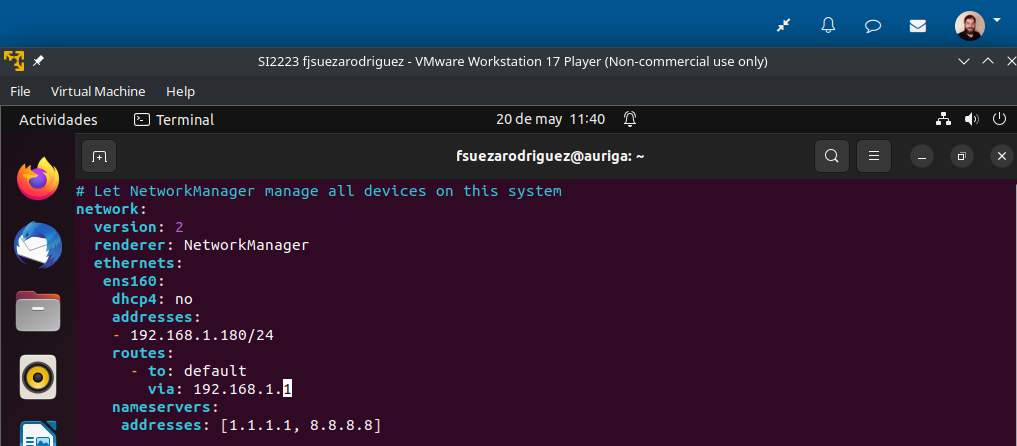
\includegraphics[scale=0.50]{netconfig-1.png}
    \caption{Configuración ip estática con Netplan}
\end{figure}

Solo un par de \textbf{comentarios} sobre la configuración que hemos puesto. La opción \textbf{gateway4} para indicar la puerta de enlace esta ya obsoleta, por lo que hemos tenido que usar \textbf{routes} con la opción \textbf{default} para indicar la puerta de enlace hacia internet. Además, hemos aprovechado para cambiar el \textbf{servidores DNS} y que nuestra interfaz use los proporcionados por \textbf{Cloudfare}, los cuales suelen ser bastante rápidos.

Tras guardar el fichero de configuración, hemos usado el comando \textbf{netplan try} para ver si la configuración es correcta, como ha sido nuestro caso.

Para comprobar que la configuración de red se ha \textbf{realizado correctamente}, hemos llevado a cabo los siguientes pasos:

\begin{enumerate}
    \item En primer lugar hemos \textbf{reiniciado} la máquina virtual, para comprobar que al reiniciarla la configuración de red es persistente, y se mantiene la dirección IP estática que le habíamos asignado.

    \item A continuación, hemos usado el comando \textbf{ip a} tanto en la \textbf{máquina virtual} como en el \textbf{SO operativo host}, que también es una Ubuntu 22.04 LTS. El resultado de ambos comandos los podemos ver en la siguientes capturas de pantalla.

    \begin{figure}[H]
        \centering
        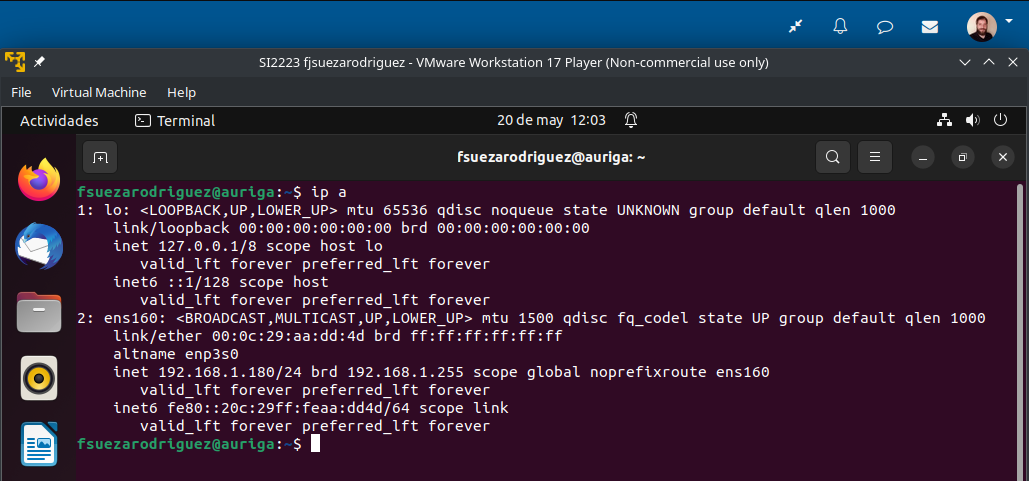
\includegraphics[scale=0.45]{netconfig-2.png}
        \caption{Configuración de red en la máquina virtual}
    \end{figure}

    \begin{figure}[H]
        \centering
        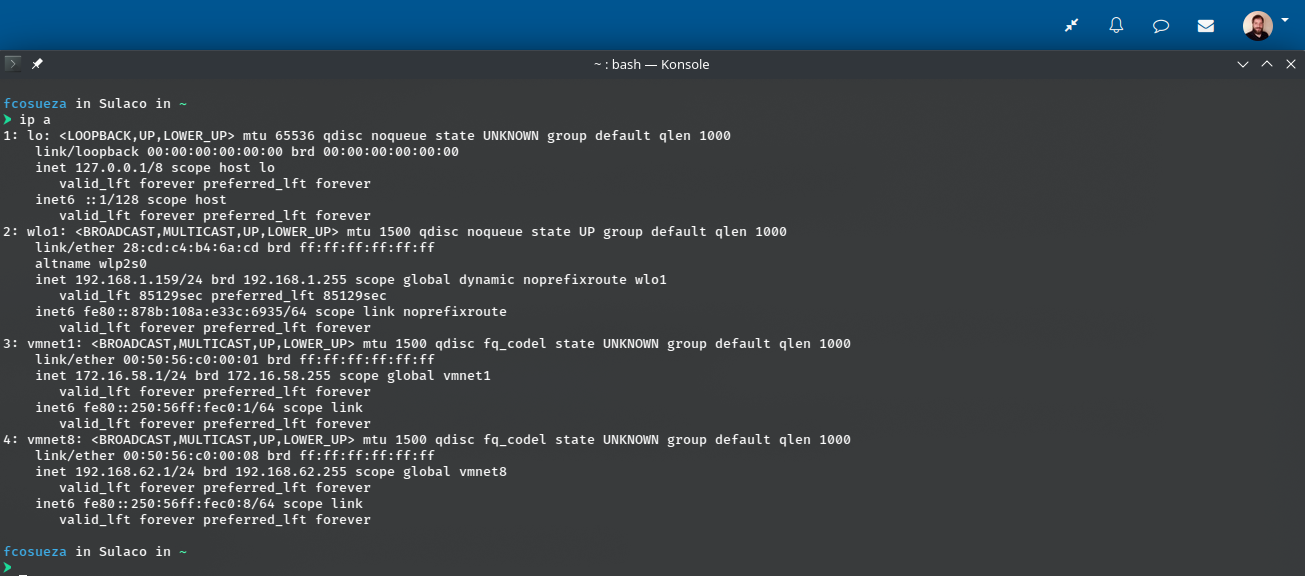
\includegraphics[scale=0.35]{netconfig-3.png}
        \caption{Configuración de red en el SO hots}
    \end{figure}

    Como vemos en la figura 2.2, la configuración de red de nuestra máquina virtual está correctamente.

    \item El siguiente paso será hacer \textbf{ping} a diferentes destinos desde la máquina virtual para comprobar que la conexión funciona correctamente. Los ping que hemos realizado son los siguientes:

    \begin{itemize}
        \item \textbf{Desde la MV a la puerta de enlace}:
        \begin{figure}[H]
            \centering
            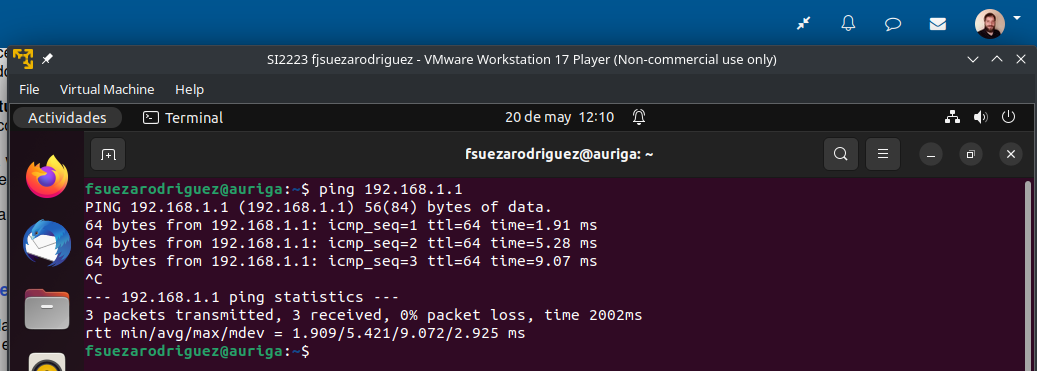
\includegraphics[scale=0.42]{ping-1.png}
            \caption{Ping desde la MV a la puerta de enlace}
        \end{figure}

        \item \textbf{Desde la máquina anfitriona a la MV}:
        \begin{figure}[H]
            \centering
            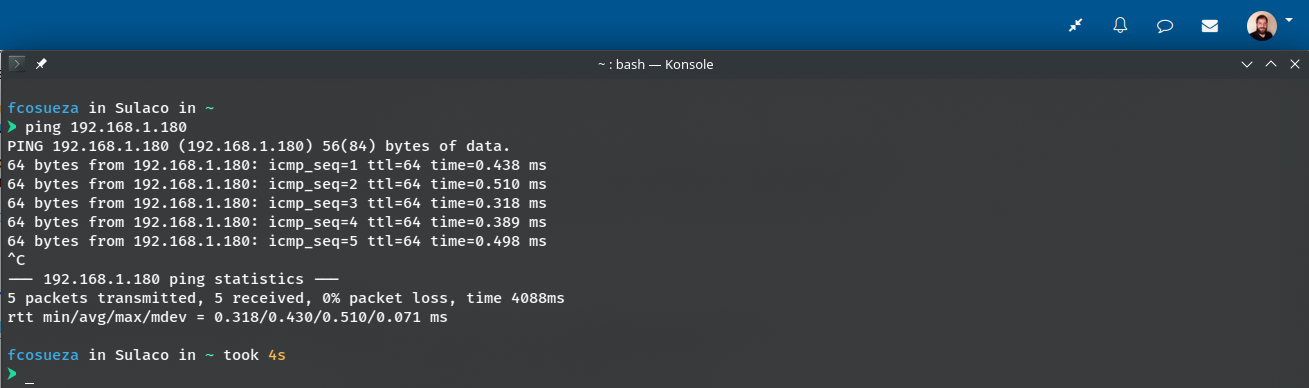
\includegraphics[scale=0.38]{ping-2.png}
            \caption{Ping desde máquina anfitriona a la MV}
        \end{figure}

        \item \textbf{Desde la MV a la máquina anfitriona}:
        \begin{figure}[H]
            \centering
            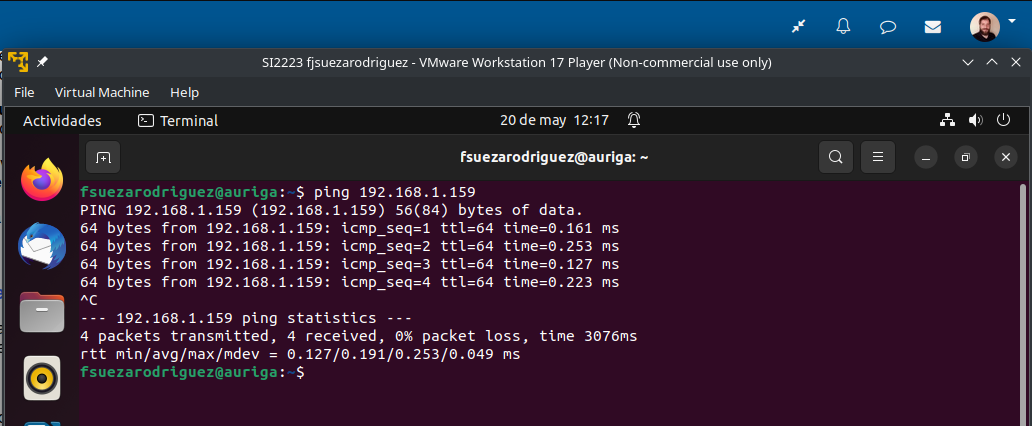
\includegraphics[scale=0.45]{ping-3.png}
            \caption{Ping desde la MV a la máquina anfitriona}
        \end{figure}
    \end{itemize}
\end{enumerate}

Como podemos comprobar, todas las conexiones funcionan correctamente en ambos sentidos. Aunque no se incluye aquí la captura, también se ha realizado ping a servidores externos a la red local desde la MV para comprobar que hay conexión a internet correctamente, siendo los resultados positivos.

\subsection{Actividad 2: Correo y Búsqueda de Información}

\subsubsection{Enunciado}
Desde la MV, haz login en el aula virtual de Sistemas Informáticos y envía a tu profesor un correo a través de la plataforma (icono del ``sobre'' a la izquierda de tu foto de perfil de usuario). El correo tendrá como asunto ``<Tu\_Nombre> Tarea 9.- Documentación de Ubuntu 22.04'', y en el cuerpo del asunto habrá un breve texto a tu elección, y se incluirá un enlace a la página oficial de documentación de Ubuntu Desktop 22.04.

Las \textbf{capturas} deben mostrar, al menos:
\begin{itemize}
    \item La página oficial de documentación de Ubuntu Desktop 22.04.
    \item El correo que se envía a través de la plataforma desde la MV redactado.
\end{itemize}

\subsubsection{Solución}
En primer lugar, hemos buscado un artículo en al documentación oficial de Ubuntu, el concreto el artículo \textbf{About Gnome}, el cual podemos ver en la siguiente captura.

\begin{figure}[H]
    \centering
    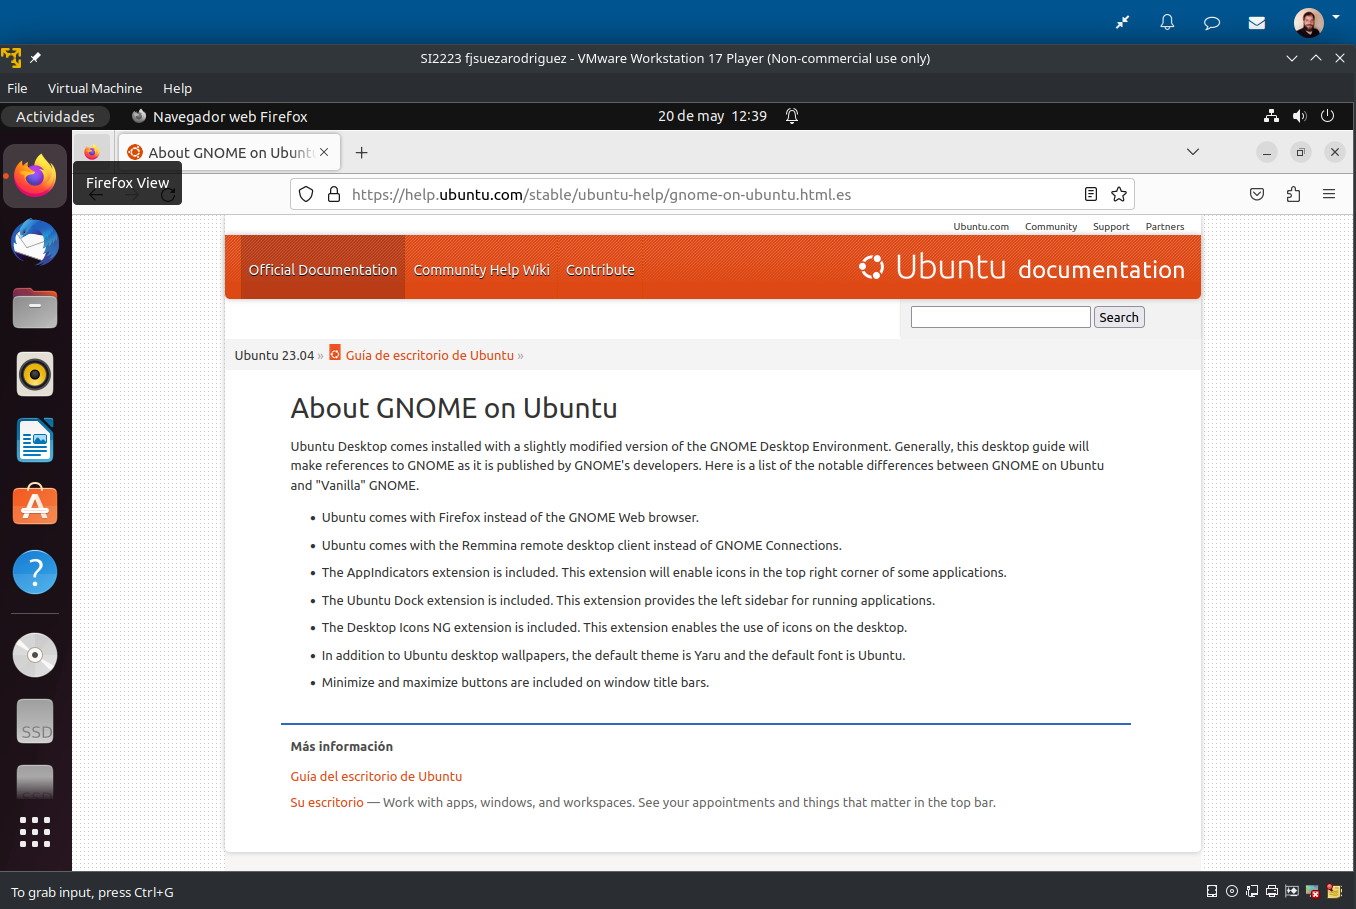
\includegraphics[scale=0.37]{ubuntuDoc.png}
    \caption{Artículo documentación oficial Ubuntu}
\end{figure}

A continuación, hemos \textbf{conectado a la plataforma} y \textbf{redactado el mensaje} al profesor con los datos que se especifican en el enunciado, como vemos a continuación.

\begin{figure}[H]
    \centering
    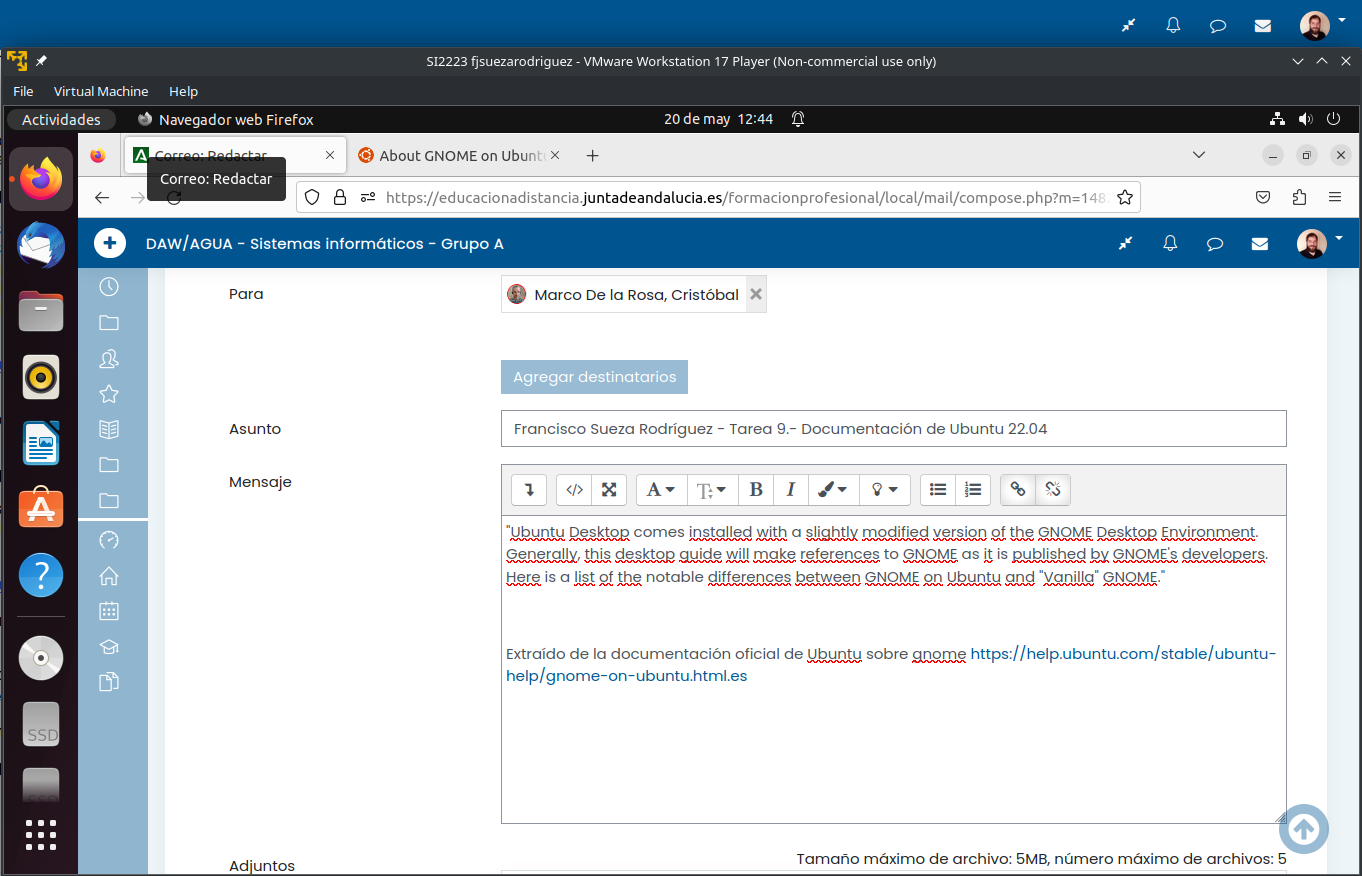
\includegraphics[scale=0.37]{emailProf.png}
    \caption{Correo desde la plataforma al profesor}
\end{figure}

\subsection{Actividad 3: Compartir recursos en la red}

\subsubsection{Enunciado}
Crea en tu máquina anfitriona una carpeta y compártela en red. A continuación, accede a dicha carpeta desde la máquina virtual Ubuntu y crea un fichero de texto nuevo en su interior con tu nombre. \textbf{Se debe hacer a través de la red local} y en ningún caso usando la opción de carpetas compartidas que ofrezca el software de virtualización usado.

Esta operación suele ser muy simple y no debería requerir ninguna instalación, pero dependiendo de qué SO tengas en tu máquina anfitriona es posible que necesites instalar en ella o en la MV distintos paquetes (Samba, NFS, APFS, etc.).

Esquema de conexión: Máquina virtual con Ubuntu > Carpeta compartida en SO anfitrión.

Las \textbf{capturas} deben mostrar, al menos:

\begin{itemize}
    \item Creación y compartición de la carpeta en la máquina real.
    \item Acceso a ella desde la MV. Se debe ver y explicar claramente cómo se ha hecho el acceso.
    \item Creación y edición de un fichero de texto desde la MV.
\end{itemize}

\subsubsection{Solución}
En este ejercicio vamos a \textbf{compartir una carpeta} entre la máquina virtual y el sistema host.

Ya que las \textbf{dos máquinas} tienen sistemas operativos \textbf{Linux}, ambas con Linuxs, vamos a usar el servidor \textbf{NFS}. Podríamos también usar Samba, pero como NFS es específico para compartir carpetas entre sistemas Linux nos hemos decantado por este.

Para \textbf{compartir la carpeta} entre los dos sistemas se han llevado a cabo los siguientes pasos:

\begin{enumerate}
    \item En primer lugar, hemos instalado el paquete \textbf{nfs-kernel-server} en la máquina anfitriona, ya que es donde vamos a crear la carpeta que se va a compartir. Esto se he realizado usando el comando \textbf{apt-get}.

    \item En segundo lugar, hemos creado la carpeta que vamos a compartir en el sistema anfitrión. En concreto, la carpeta creada ha sido \textbf{/mnt/miCarpeta}. Para ello sea ha usado el comando \textbf{mkdir}, como podemos ver en la siguiente captura.

    \begin{figure}[H]
        \centering
        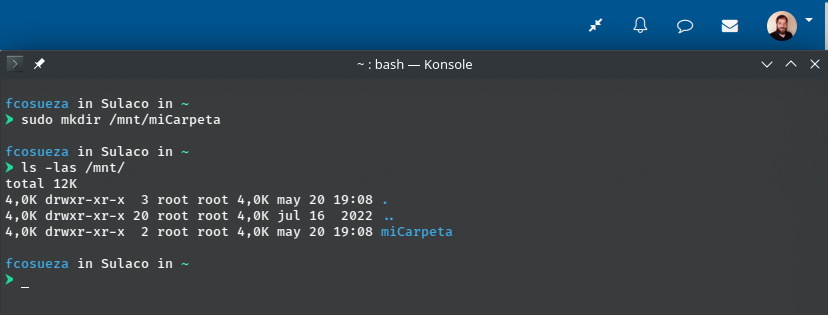
\includegraphics[scale=0.45]{nfs-1.png}
        \caption{Creación de la carpeta compartida}
    \end{figure}

    \item A continuación hemos editado el archivo \textbf{/etc/exports}, para permitir el acceso a la carpeta compartida que hemos creado desde la máquina virtual. Para ello, hemos añadido la siguiente línea:
    \begin{figure}[H]
        \begin{tcolorbox}[sharp corners, colback=yellow!30, colframe=white!20]
            \scriptsize
            \begin{verbatim}
/mnt/miCarpeta 192.168.1.180/24(rw,async,no_subtree_check,root_squash)\end{verbatim}
        \end{tcolorbox}
    \end{figure}

    \item Como \textbf{último paso} en el \textbf{sistema anfitrión}, hemos montado el sistema \textbf{exportfs} y \textbf{reiniciado el servicio nfs}, usando el comando \textbf{systemctl restart nfs-kernel-server}. Tras esto, nuestra carpeta estará creada correctamente y compartiéndose en la red local, como podemos ver en la siguiente captura.

    \begin{figure}[H]
        \centering
        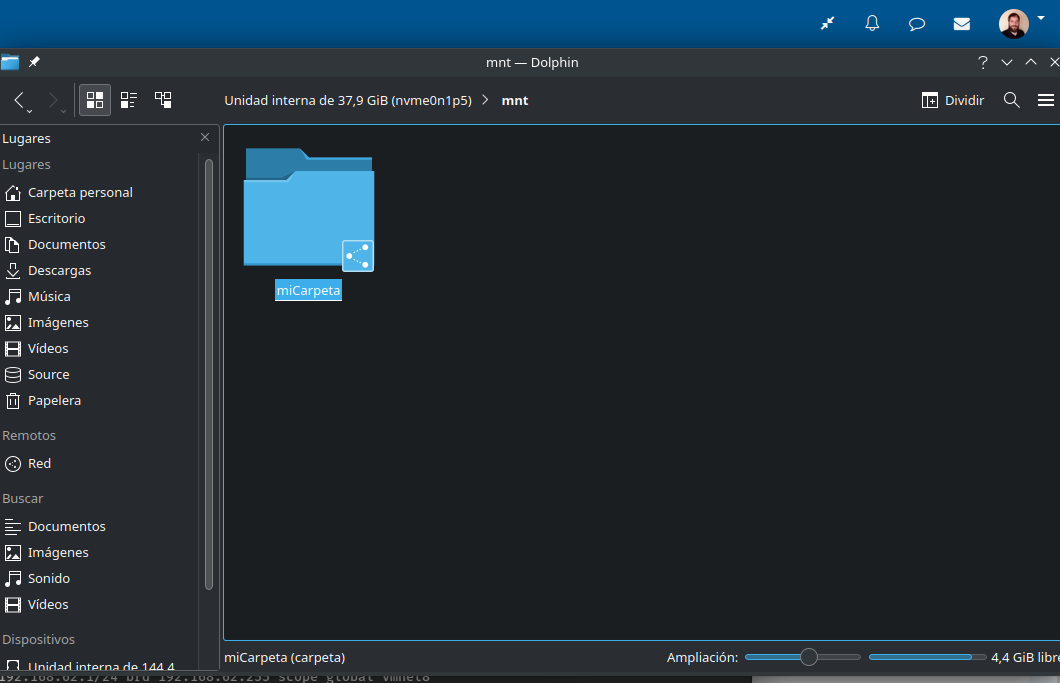
\includegraphics[scale=0.45]{nfs-2.png}
        \caption{Carpeta creada y compartiéndose en el anfitrión}
    \end{figure}

    \item Para poder \textbf{acceder desde el cliente} (nuestra máquina virtual), en primer lugar debemos instalar el paquete \textbf{nfs-common}, lo cual hemos llevado a cabo usando el comando \textbf{apt-get}.

    \item A continuación hemos creado la carpeta \textbf{/mnt/miCarpeta-local}, que será el punto donde montaremos la carpeta compartida, para poder acceder a ella de forma local como si estuviera en nuestro propio ordenador.

    Este tipo de acceso de más sencillo de realizar en NFS que en Samba, que tiene más restricciones, uno de los motivos por los cuales hemos elegido NFS.

    \item El siguiente paso ha sido \textbf{montar la carpeta remota} en el directorio que hemos creado, usando para ello el comando \textbf{mount -t nfs 192.168.1.159:/mnt/miCarpeta /mnt/miCarpeta-local}. Con esto, ya tenemos montada la carpeta remota en nuestro sistema con permisos de escritura y de lectura.

    \item Para comprobar que todo funciona correctamente, hemos creado un fichero de texto simple usando el comando \textbf{echo} y redireccionando la salida a un fichero de texto desde nuestra máquina virtual, como podemos ver en la siguiente captura.

    \begin{figure}[H]
        \centering
        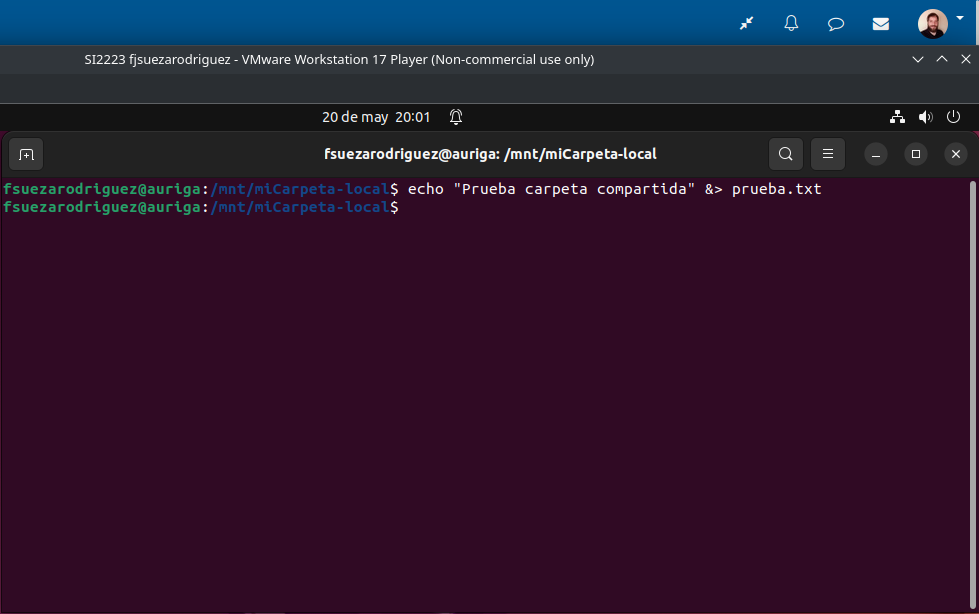
\includegraphics[scale=0.45]{nfs-3.png}
        \caption{Creación de un fichero de texto en la carpeta compartida}
    \end{figure}

    \item Por último, hemos leído el fichero de texto desde la máquina anfitrión para comprobar que se ha creado correctamente. Hemos usado el comando \textbf{cat} desde la terminal, como vemos a continuación.

    \begin{figure}[H]
        \centering
        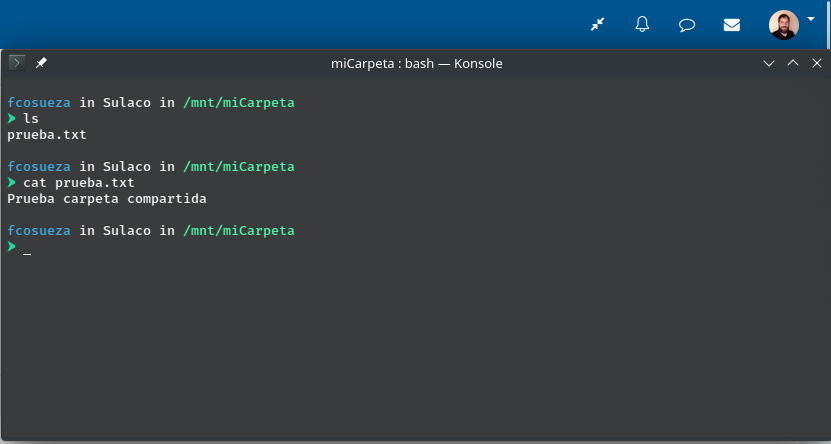
\includegraphics[scale=0.55]{nfs-4.png}
        \caption{Lectura del fichero desde la máquina anfitrión}
    \end{figure}
\end{enumerate}

\subsection{Actividad 4: Conexión Remota a Dispositivos}

\subsubsection{Enunciado}
Realiza conexiones remotas desde el SO anfitrión (cliente) a la MV de Ubuntu (servidor) usando dos mecanismos:

\begin{itemize}
    \item SSH. Comenta las ventajas de utilizar SSH frente a Telnet.
    \item VNC.
\end{itemize}

Esquema de conexión 1: Cliente SSH en la máquina anfitriona > Servidor SSH en MV Ubuntu.
Esquema de conexión 2: Cliente de VNC en la máquina anfitriona > Servidor VNC en MV Ubuntu.

Las \textbf{capturas} deben mostrar, al menos:
\begin{itemize}
    \item Ventana de conexión del cliente SSH en la máquina anfitriona.
    \item Sesión SSH ya conectada y funcionando.
    \item Configuración de compartición de pantalla en la MV para el acceso mediante VNC.
    \item Ventana de conexión del cliente VNC en la máquina anfitriona.
    \item Sesión VNC ya conectada y funcionando.
\end{itemize}

\subsubsection{Solución}
En este ejercicio vamos a realizar una conexión remota desde la máquina anfitriona a la máquina virtual de dos formas diferentes. En primer lugar, usaremos \textbf{ssh} (Secure Shell) y a continuación usaremos \textbf{VCN} (Virtual Network Computing).

\begin{itemize}
    \item \textbf{Conexión con SSH}

    Para realizar este tipo de conexión entre las dos máquinas nos necesitamos realizar ninguna configuración especial en ningunas de ellas. La aplicación \textbf{OpenSSH} viene \textbf{instalada por defecto} en todas las distribuciones Linux y además esta configurado por defecto para los casos básicos. Lo único que deberíamos hacer es inicializar el servicio en la máquina virtual empleando el comando \textbf{systemctl}.

    Una vez inicializado el servicio en la MV, desde la máquina anfitriona solo deberíamos realizar la conexión, utilizando el comando \textbf{ssh fsuezarodriguez@192.168.1.180}, como podemos ver en la siguiente captura de pantalla.

    \begin{figure}[H]
        \centering
        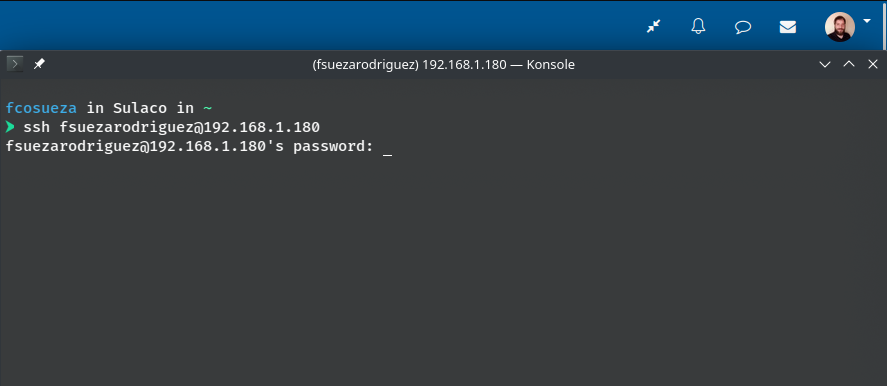
\includegraphics[scale=0.55]{ssh-1.png}
        \caption{Ventana de conexión del cliente SSH}
    \end{figure}

    Para realizar la conexión, nos pedirá la \textbf{contraseña del usuario} que hemos indicado. Una vez introducida la contraseña, se realizará la conexión situándonos en el directorio home del usuario.

    En la siguiente captura podemos ver como se ha establecido la conexión y hemos realizado un listado de los archivos en el directorio del usuario fsuezarodriguez. Podemos ver además como el prompt ha cambiado y nos muestra que estamos trabajando con el \textbf{usuario fsuezarodriguez} en el \textbf{host auriga}.

    \begin{figure}[H]
        \centering
        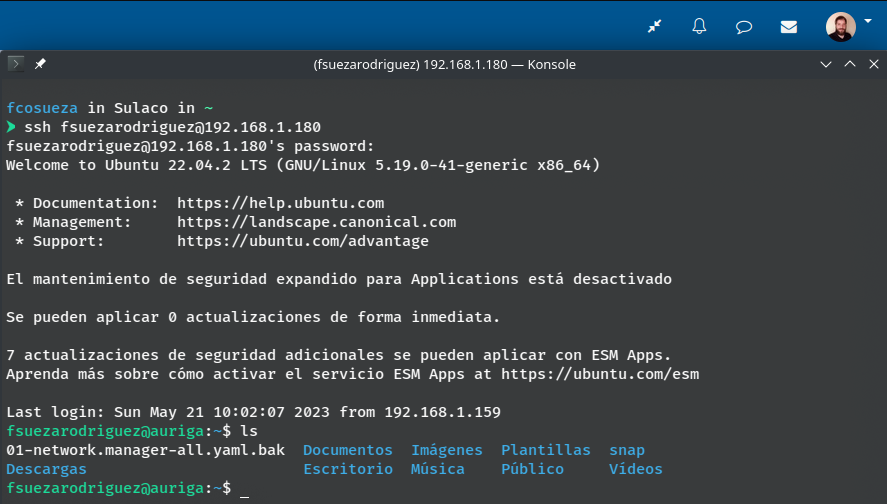
\includegraphics[scale=0.55]{ssh-2.png}
        \caption{Conexión realiza con ssh a la MV}
    \end{figure}

    \item \textbf{Conexión con VNC}

    Ahora vamos a realizar una conexión utilizando el protocolo \textbf{VNC}, que nos permite conectarnos de forma remota al escritorio de la máquina servidor y manejarlo. Al igual que en el punto anterior, no vamos a tener que realizar instalación de ninguna aplicación, ya que las que vamos a usar, \textbf{vino} (servidor) y \textbf{remmina} ya vienen instaladas por defecto.

    En primer lugar, hemos realizado la \textbf{configuración} del acceso remoto mediante VNC en Ubuntu, que se realiza accediendo a \textit{\textbf{Configuración}-->\textbf{Compartir}}, como podemos ver en la siguiente captura.

    \begin{figure}[H]
        \centering
        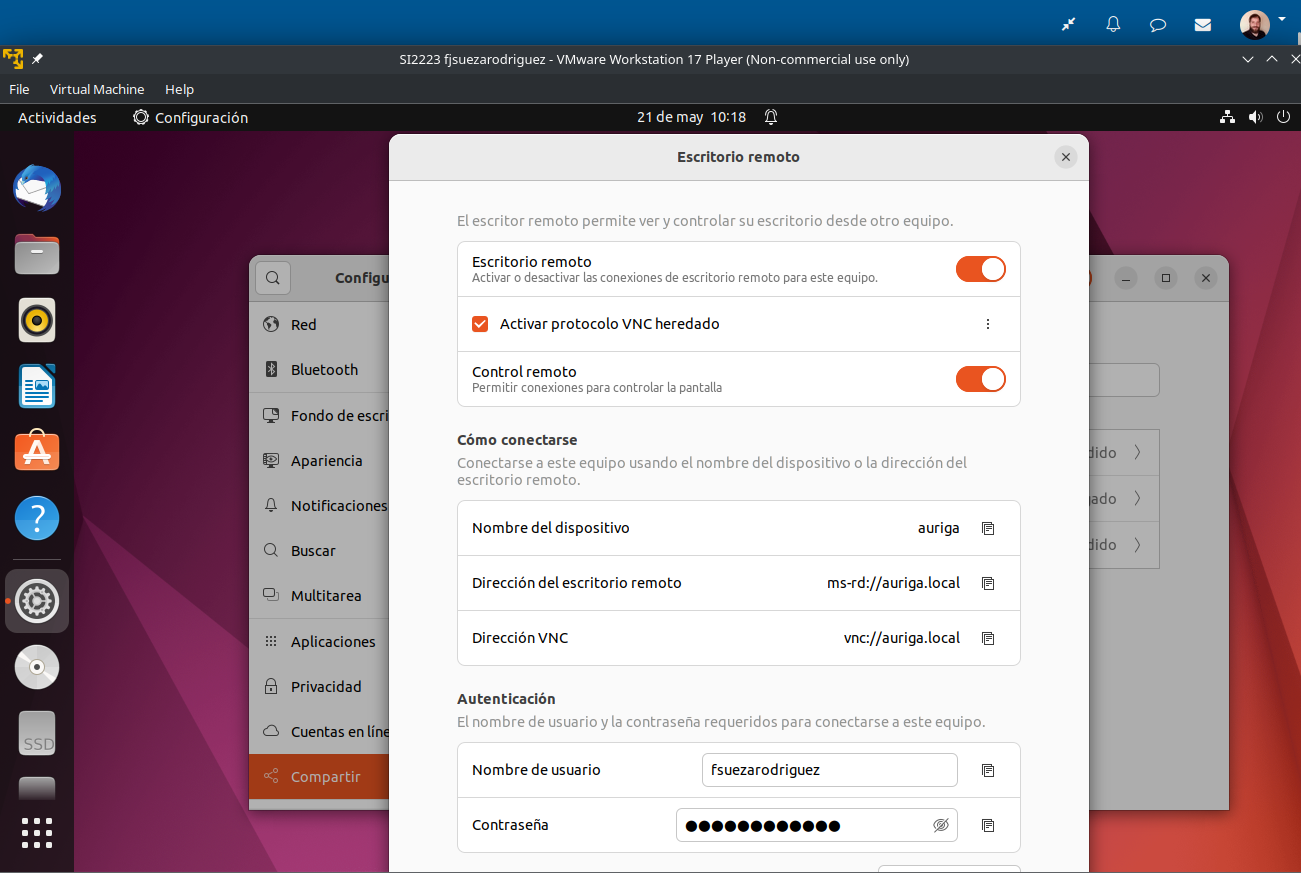
\includegraphics[scale=0.33]{vnc-1.png}
        \caption{Configuración del servidor de VNC en Gnome}
    \end{figure}

    En la \textbf{máquina anfitrión} vamos a usar \textbf{KRDC}, ya la distribución que se usa en esta máquina es \textbf{Kubuntu 22.04 LTS} y es la aplicación que viene por defecto instalada.

    En la siguiente captura podemos ver la \textbf{configuración de la conexión desde KRDC}, como vemos nos ofrece diferentes opciones, incluía usar ssh tunneling para realizar la conexión cifrada.

    \begin{figure}[H]
        \centering
        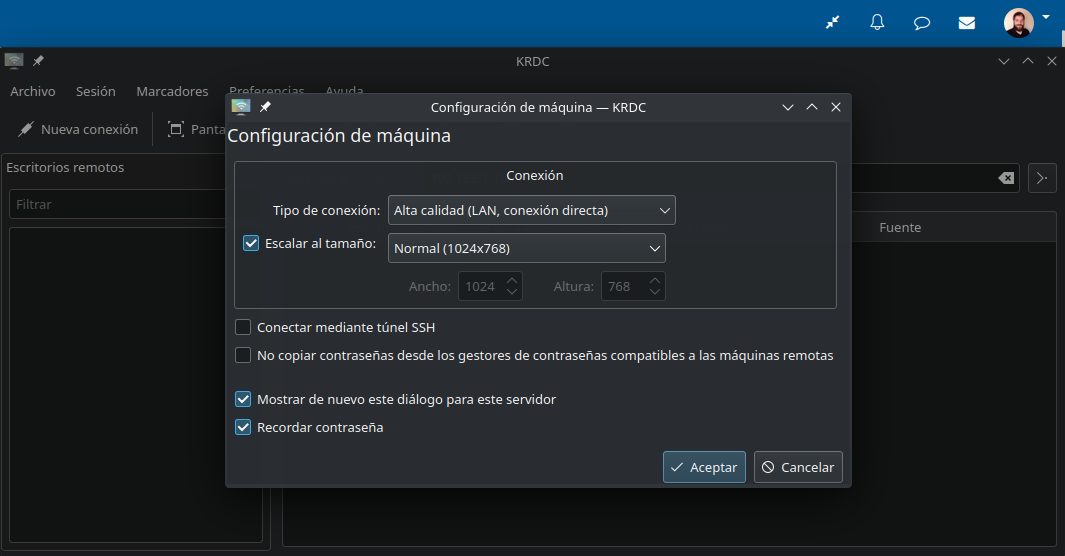
\includegraphics[scale=0.40]{vnc-2.png}
        \caption{Configuración de la conexión con KRDC}
    \end{figure}

    Una vez introducidos los datos de configuración que queramos, pulsamos en aceptar y tras pedirnos la contraseña, que deberemos introducir la que hayamos establecido en la máquina virtual, la \textbf{conexión se realizará con éxito}, si hemos hecho todo bien, como vemos en la siguiente imagen.

    \begin{figure}[H]
        \centering
        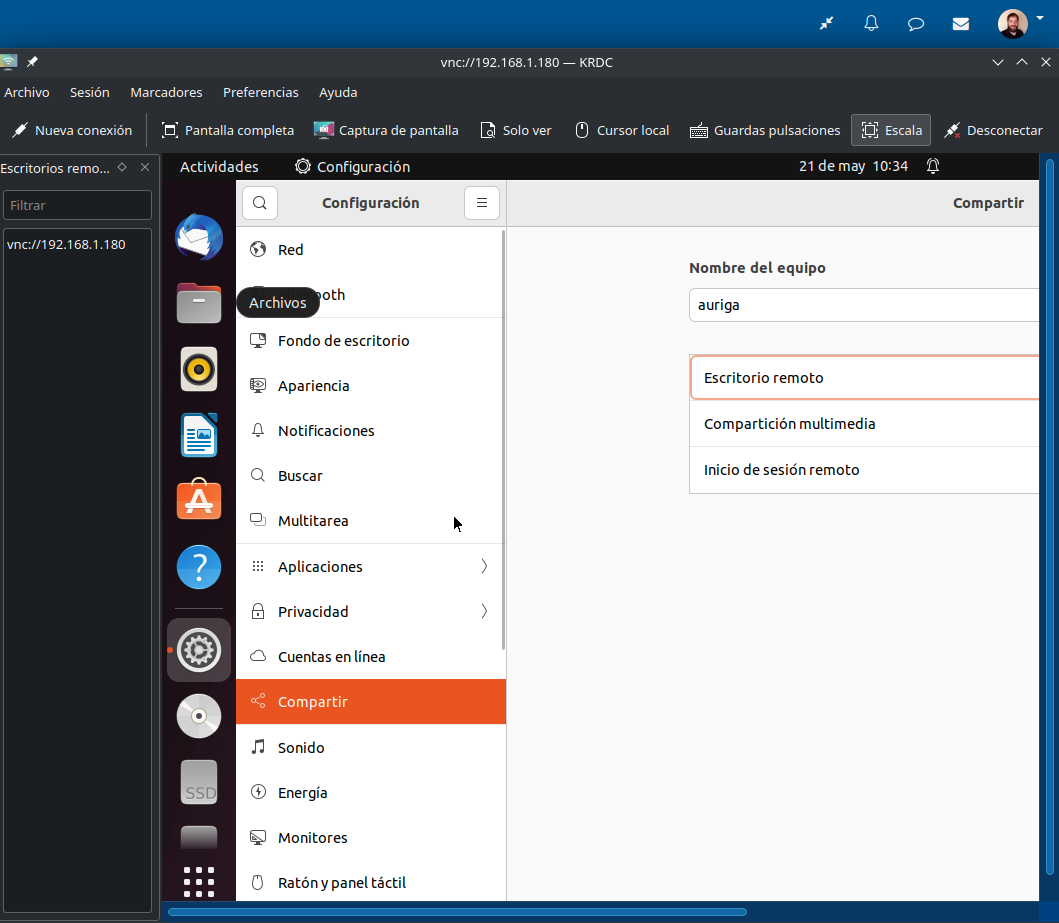
\includegraphics[scale=0.40]{vnc-3.png}
        \caption{Conexión realizada desde la máquina anfitriona con KRDC}
    \end{figure}
\end{itemize}

\subsection{Actividad 5: Servicio FTP}

\subsubsection{Enunciado}
Instala en la MV de Ubuntu un servidor FTP y en el SO anfitrión un cliente FTP como Filezilla, para acceder desde él al servidor. Una vez esté todo instalado, realiza una transmisión de algún archivo desde el cliente FTP al servidor y viceversa. Muestra los mensajes del cliente FTP en los que se confirma que la descarga y subida se han realizado correctamente.

Esquema de conexión: Cliente FTP en SO anfitrión > Servidor FTP en MV Ubuntu.

Las \textbf{capturas} deben mostrar, al menos:

\begin{itemize}
    \item Instalación servidor FTP en MV Ubuntu.
    \item Configuración del servidor FTP con los permisos necesarios para permitir acceso de lectura y escritura.
    \item Conexión desde el cliente FTP en la máquina anfitriona.
    \item Una descarga y una subida correctas.
\end{itemize}

\subsubsection{Solución}
Ahora vamos a montar un \textbf{servidor FTP} en la máquina virtual y vamos a acceder a él desde la máquina anfitriona. En el lado del servidor, vamos a instalar \textbf{vsftpd}, un servidor FTP ligero, robusto y fácil de configurar. En el lado del cliente vamos a usar \textbf{Filezilla}, uno de los clientes más usados.

Para llevar a cabo todo este proceso vamos a realizar los siguiente pasos:

\begin{enumerate}
    \item En primer lugar, vamos a \textbf{instalar vsftpd} en la máquina virtual, para lo que vamos a usar \textbf{apt-get}, como vemos en la siguiente captura.

    \begin{figure}[H]
        \centering
        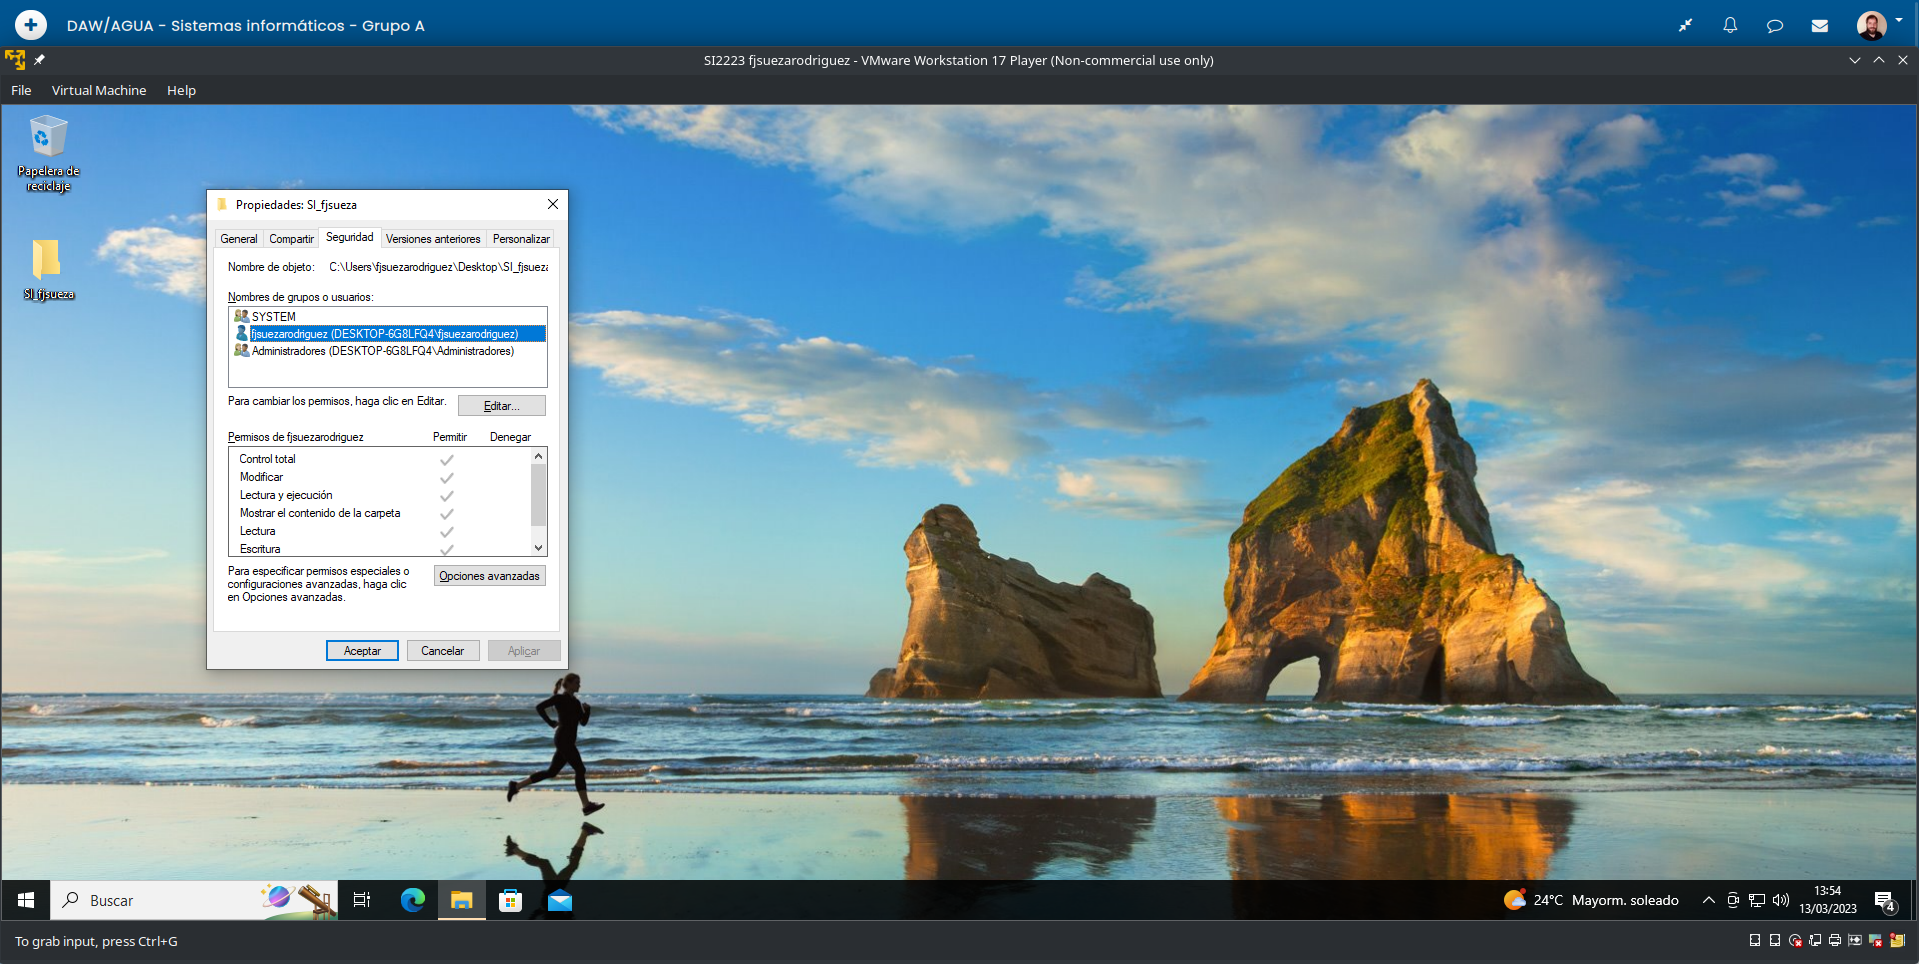
\includegraphics[scale=0.58]{ftp-1.png}
        \caption{Instalación de vsftpd en la máquina virtual}
    \end{figure}

    \item El siguiente paso es \textbf{configurar el servidor FTP}, lo que vamos a hacer editando el \textbf{archivo de configuración} de vsftpd, que editaremos con el editor de textos \textbf{vim}, como vemos en la siguiente captura.

    \begin{figure}[H]
        \centering
        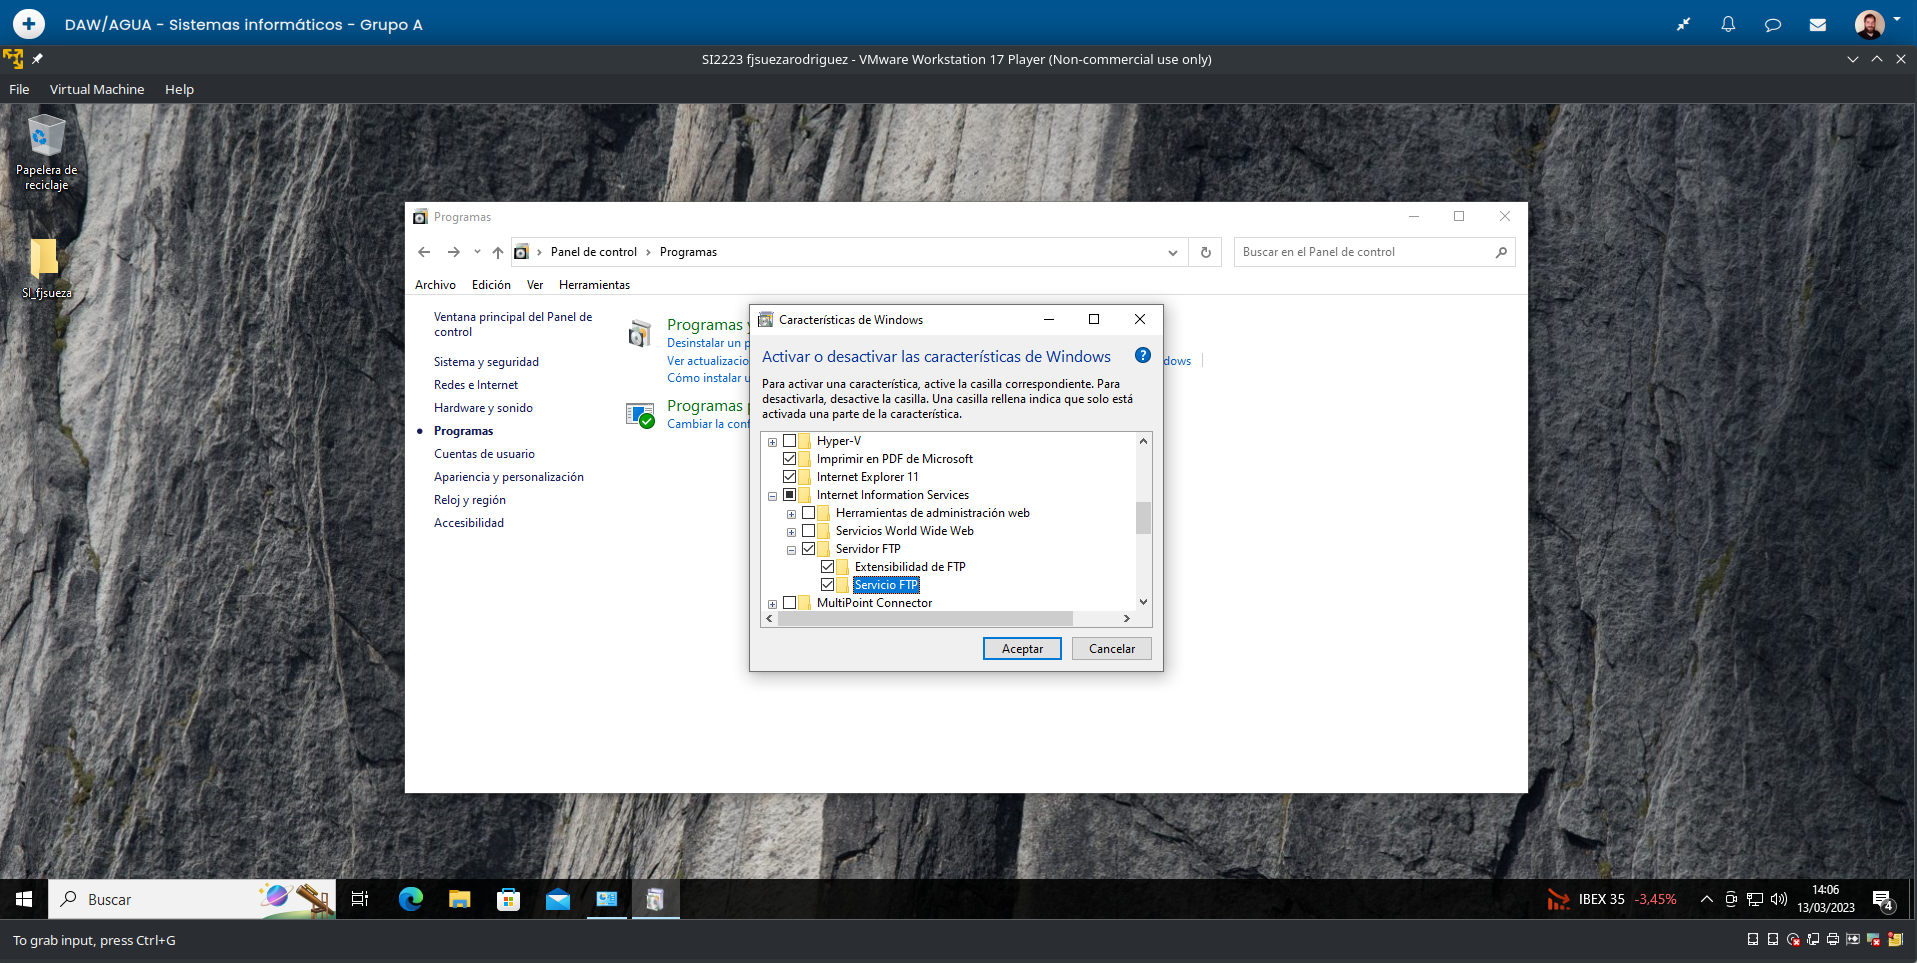
\includegraphics[scale=0.58]{ftp-2.png}
        \caption{Configuración de vsftpd}
    \end{figure}

    A la hora de configurar el servidor, hemos decidido usar como \textbf{usuario} el que ya teníamos creado en la máquina virtual, esto es, \textbf{fsuezarodriguez}, por lo que al conectar desde la máquina anfitrión apareceremos en el directorio \textbf{/home/fsuezarodríguez}.

    Podríamos haber creado otro usuario, llamado, por ejemplo, ftp, pero con el usuario que tenemos ya nos vale para lo que queremos hacer. Además, así nos evitamos complicar el proceso ya que habría que crear el usuario, grupo, modificar ciertos archivos, etc...

    Las principales opciones que hemos usado en la configuración son las siguientes:
    \begin{itemize}
        \item \textbf{listen=NO}: no queremos que el servidor se ejecute al inicio, sino ejecutarlo nosotros manualmente. Es una cuestión de preferencias, pero si el servidor va a estar continuamente activo esta opción debería tener el valor \textbf{YES}.

        \item \textbf{listen\_ipv6=YES}: con esta opción habilitamos la escucha en los sockets ipv6 y ipv4, para que acepte conexión tanto de una versión del protocolo como del otro.

        \item \textbf{anoymous\_enable=NO}: con esta opción deshabilitamos el acceso anónimo al servidor.

        \item \textbf{write\_enable=YES}: aquí estamos concediendo permisos de escritura al usuario del ftp. En el caso de que solo ofreciéramos archivos para descarga, esta opción tendría que tener el valor \textbf{NO}.

        \item \textbf{local\_umask=022}: con esta directiva estamos estableciendo que los archivos creados por lo usuarios tengan los \textbf{permisos 755}. Es una de las configuraciones mas usuales en los FTPs y con ello nos aseguramos de que cuando un usuario crea un archivo, no pueda ser borrado por otros usuarios, aunque si puede ser ejecutado y leído por estos.
    \end{itemize}

    Aunque hay más opciones, estas podríamos decir que son las más importantes.

    \item El siguiente paso es \textbf{realizar una conexión} desde la máquina anfitriona al FTP. Para ello, como hemos comentado anteriormente, vamos a usar \textbf{Filezilla}.

    Una vez introducidos los datos de conexión, usuario, servidor, contraseña, etc.., pulsamos en \textbf{conexión rápida} y la conexión se realizará correctamente, como podemos ver en la siguiente captura.

    \begin{figure}[H]
        \centering
        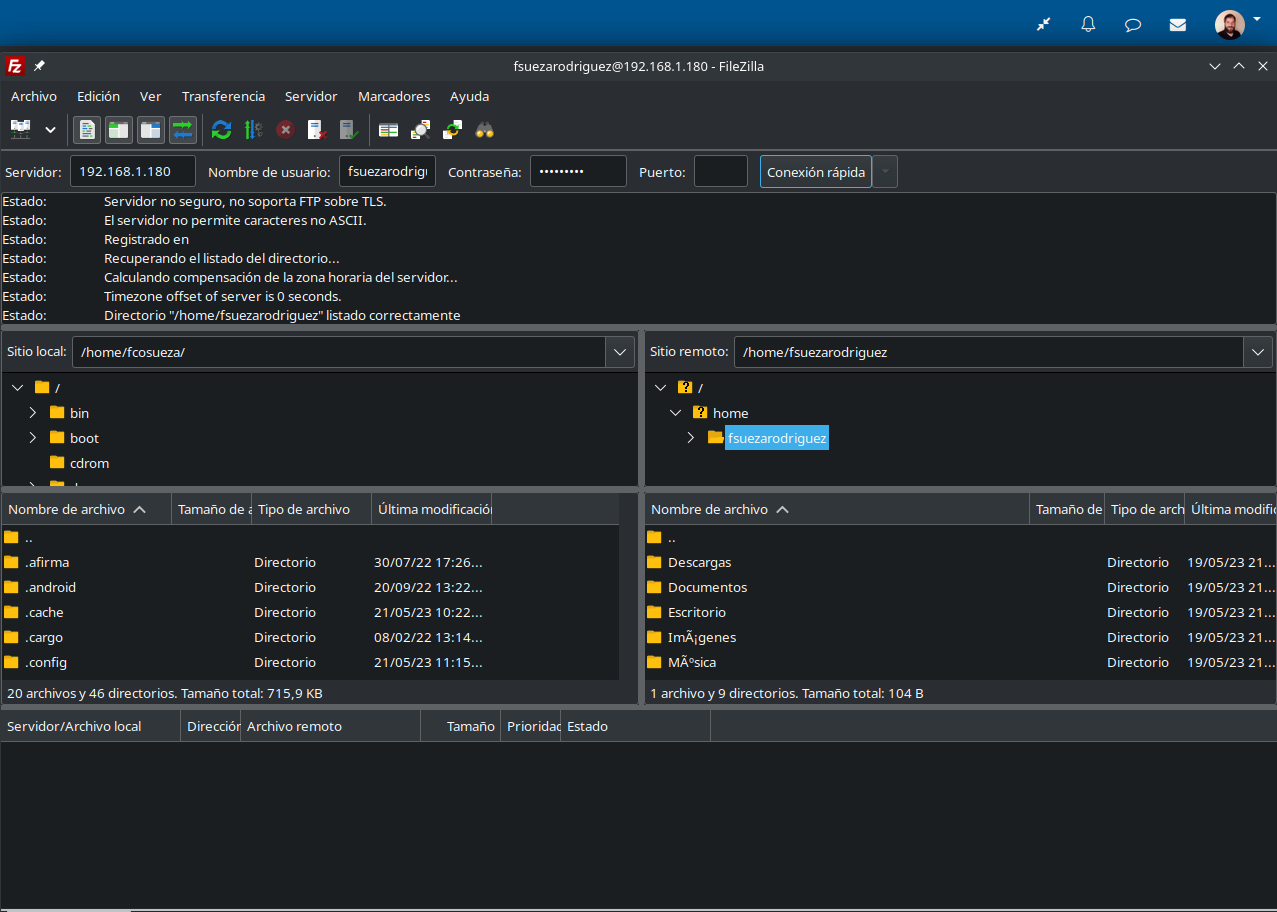
\includegraphics[scale=0.50]{ftp-3.png}
        \caption{Conexión al FTP con Filezilla desde la máquina anfitrión}
    \end{figure}

    \item Como \textbf{último paso}, vamos a crear un fichero de texto, llamado \textbf{archivo.txt}, en el directorio del FTP desde la máquina virtual, para realizar su descarga desde Filezilla.

    Al mismo tiempo, hemos creado otro archivo de texto en la \textbf{máquina anfitriona}, llamado \textbf{subida.txt}, que subiremos al servidor FTP usando también Filezilla.

    En la siguiente captura, podemos ver como las dos operaciones (subida y bajada), se han realizado con éxito.

    \begin{figure}[H]
        \centering
        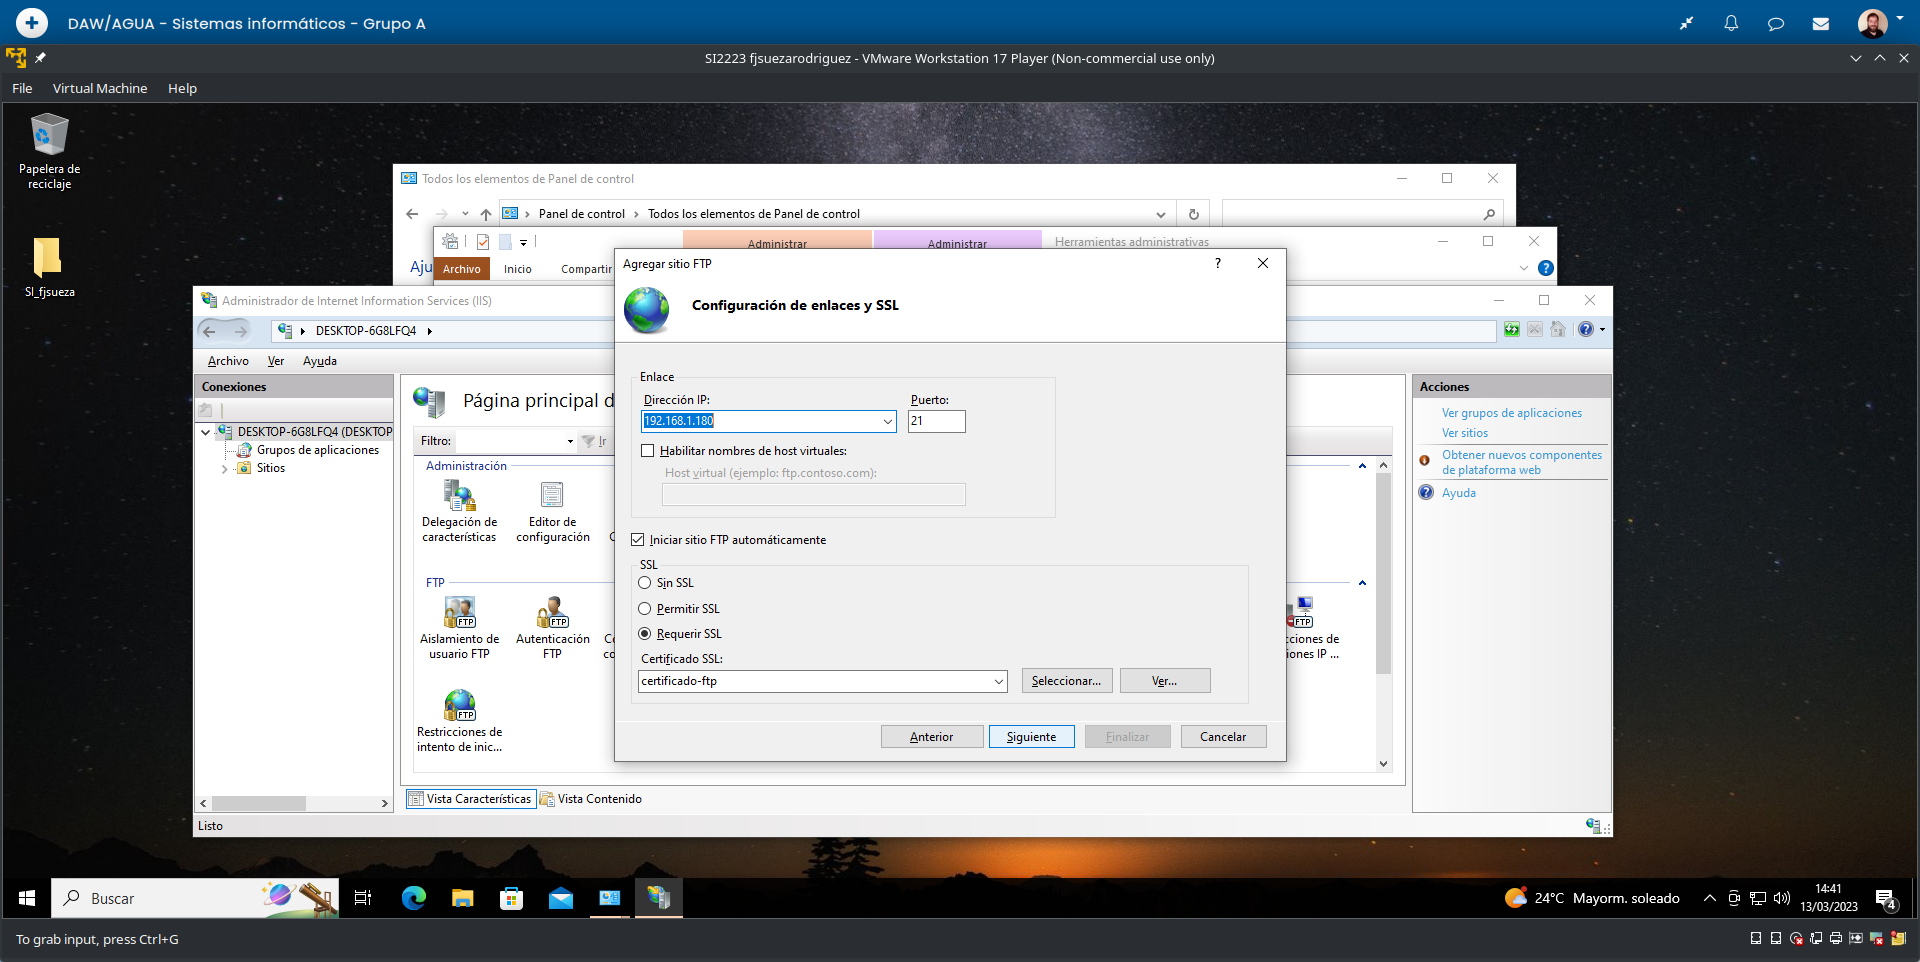
\includegraphics[scale=0.45]{ftp-4.png}
        \caption{Descarga y Subida de archivos con Filezilla}
    \end{figure}
\end{enumerate}

\subsection{Actividad 6: Servidor Web}

\subsubsection{Enunciado}
Instala el servidor web Apache en la MV de Ubuntu y configúralo para que se inicie automáticamente al iniciar Ubuntu. A continuación, en el SO anfitrión abre en un navegador la página web miprimeraweb.html que creaste en la tarea 6. Para ello previamente tendrás que copiar dicha página web en el directorio correspondiente del servidor Apache que has instalado.

Si no realizaste la actividad donde se creaba esta página web, a continuación se detalla el código de la misma que deberás crear y guardar en el archivo miprimeraweb.html. Para ello utiliza un editor de texto de Ubuntu y en la imagen no olvides poner tu foto.

\begin{figure}[H]
    \centering
    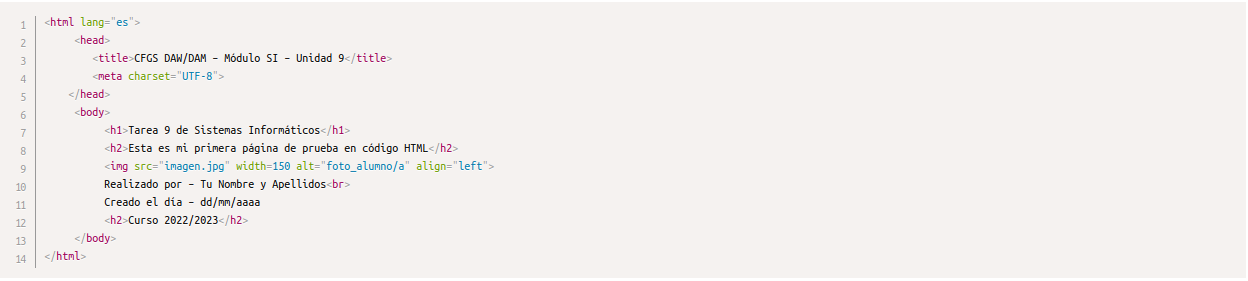
\includegraphics[scale=0.50]{web-html.png}
    \caption{Página web de ejemplo}
\end{figure}

Esquema de conexión: Navegador web en la máquina anfitriona > Servidor Apache en MV Ubuntu.

Las \textbf{capturas} deben mostrar, al menos:

\begin{itemize}
    \item Instalación de Apache en la MV.
    \item Habilitar el servicio Apache para que se inicie automáticamente con el inicio de Ubuntu.
    \item Archivos de la página web copiados al directorio correspondiente de Apache (comentar/corregir permisos si es necesario).
    \item Acceso a la página web desde el navegador web en la máquina anfitriona (comentar/corregir permisos si es necesario).
\end{itemize}

\subsubsection{Solución}
Por último, vamos a \textbf{instalar} y \textbf{desplegar un servidor web} en la máquina virtual, usando el servidor \textbf{Apache}, uno de los servidores web más utilizados. La página web que vamos a servir es \textbf{HTML} plano, por lo que no será necesario instalar PHP. Los pasos que hemos seguido son los siguientes:

\begin{enumerate}
    \item En primer lugar, hemos \textbf{instalado Apache2} en la máquina virtual, usando el comando \textbf{apt-get}, como vemos en la siguiente figura.

    \begin{figure}[H]
        \centering
        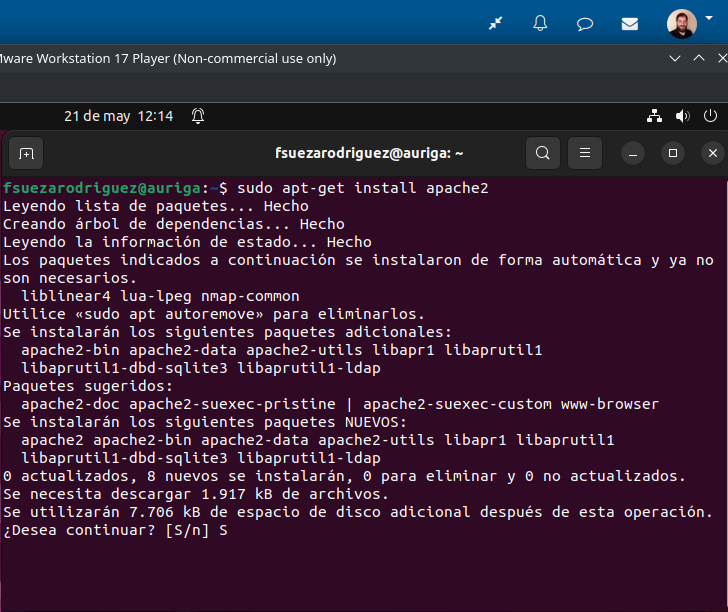
\includegraphics[scale=0.60]{web-1.png}
        \caption{Instalación de Apache en la máquina virtual}
    \end{figure}

    \item Una vez que se ha instalado correctamente, vamos a indicar que se ejecute el servidor cada vez que se iniciar el sistema operativo. Podríamos usar \textbf{sysv-rc-conf}, pero Apache tiene muy buena integración con \textbf{systemd}, por lo que su manejo es mucho más rápido usando los comandos \textbf{service} ó \textbf{systemctl}. Nosotros, vamos a usar \textbf{systemctl} para iniciar Apache cada vez que se inicie la máquina.

    Para ello, vamos a usar el comando\textbf{systemctl enable apache2.service}, como podemos ver en la siguiente captura.

    \begin{figure}[H]
        \centering
        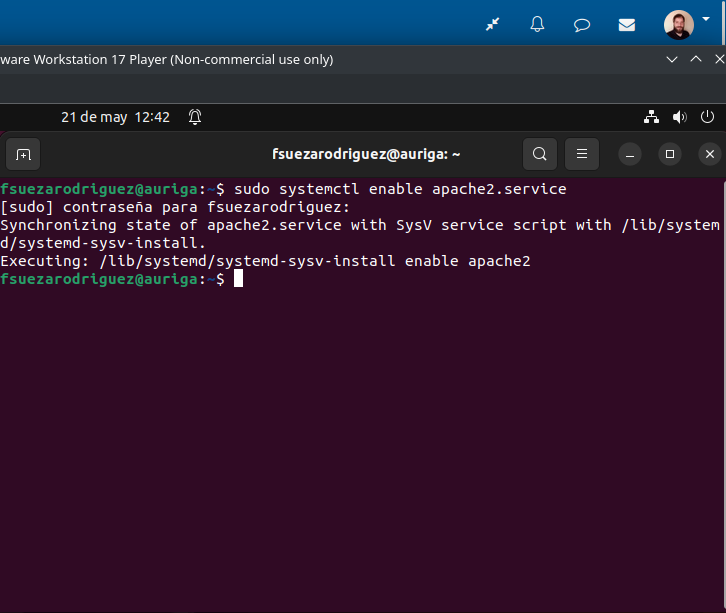
\includegraphics[scale=0.60]{web-2.png}
        \caption{Habilitación de Apache para que se ejecute al inicio}
    \end{figure}

    \item Respecto a la \textbf{configuración}, no hay mucho que comentar, ya que vamos a usar la que viene por defecto, porque no necesitamos ninguna configuración especial.

    \item El siguiente punto es \textbf{copiar el archivo HTML} con nuestra página web y nuestra foto en el directorio \textbf{/var/www/html}. Además, cambiaremos el propietario a root, si no estuvieran ya así y los permisos a \textbf{755}, para que solo root pueda eliminar o modificar nuestra página web.

    \begin{figure}[H]
        \centering
        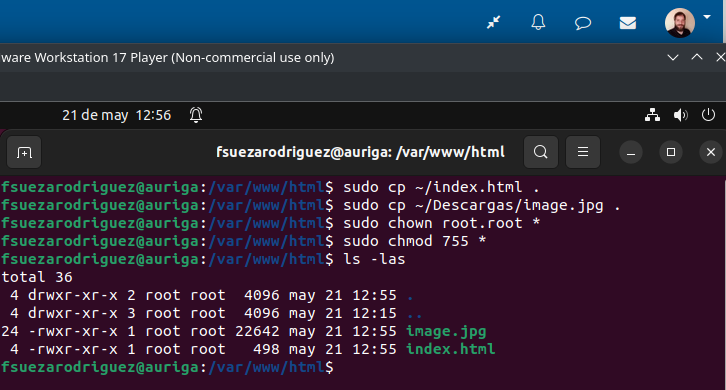
\includegraphics[scale=0.60]{web-3.png}
        \caption{Copia de index.html y cambio de permisos}
    \end{figure}

    \item Por último, vamos a \textbf{acceder a la página web} desde la \textbf{máquina anfitriona}. Como podemos ver, la página se ve correctamente, por lo que el servidor esta funcionando a la perfección.

    \begin{figure}[H]
        \centering
        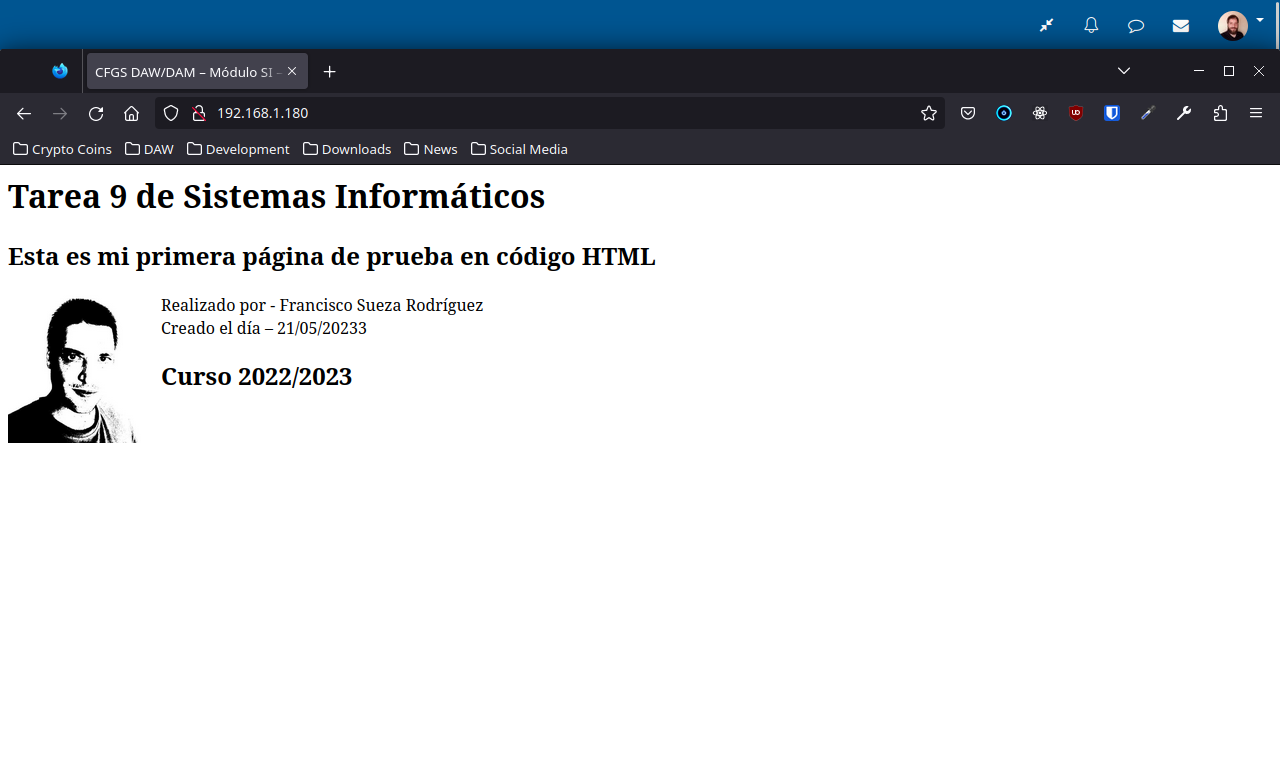
\includegraphics[scale=0.45]{web-4.png}
        \caption{Acceso a la página web desde el anfitrión}
    \end{figure}
\end{enumerate}





% Bibliography

%\newpage
%\bibliography{citas}
%\bibliographystyle{unsrt}

\end{document}